
\documentclass[11pt]{article}
\usepackage[hmargin=1.5cm,vmargin=1.5cm]{geometry}

\usepackage[affil-it]{authblk}

\usepackage{ifpdf}
\ifpdf 
    \usepackage[pdftex]{graphicx}   % to include graphics
    \pdfcompresslevel=9 
    \usepackage[pdftex,     % sets up hyperref to use pdftex driver
            plainpages=false,   % allows page i and 1 to exist in the same document
            breaklinks=true,    % link texts can be broken at the end of line
            colorlinks=true,
            pdftitle=My Document
            pdfauthor=My Good Self
           ]{hyperref} 
    \usepackage{thumbpdf}
\else 
    \usepackage{graphicx}       % to include graphics
    \usepackage{hyperref}       % to simplify the use of \href
\fi 

\title{Fast Timing Sexy Title}

\author[1]{D.~Anderson, A.~Apresyan, A.~Bornheim, J.~Duarte, C.~Pena, M.~Spiropulu, S.~Xie}
\author[2]{A.~Ronzhin}
\affil[1]{California Institute of Technology, Pasadena, CA, USA}
\affil[2]{Fermi National Accelerator Laboratory, Batavia, USA}

\date{}

\begin{document}

\maketitle
\abstract{ Current and future high energy physics particle colliders are capable
to provide instantaneous luminosities of 10$^{34}$ cm$^{-2}$s$^{-1}$ and above.
The high center of mass energy, large number of simultaneous collision of beam
particles in the experiments and the very high repetition rates of the collision
events pose huge challenges. They result in extremely high particle fluxes,
causing very high occupancies in the particle physics detectors operating at
these machines. We discuss how timing information with a precision of around 10
ps and below can aid the reconstruction of the physics events under such
challenging conditions. 

We present studies and measurements from test beams and GEANT4 simulations for
calorimeter based timing measurements to explore the ultimate timing precision
achievable for high-energy photons. We put particular focus on techniques to
measure the timing with a precision of about 10 ps in association with the
energy of the photon. We present studies with detector prototypes where we
achieve the timing resolution of a few tens of picoseconds in test beam
measurements. Finally, possible applications of precision timing in
future high-energy physics experiments are discussed. }



\section{Introduction}
Current and future high energy physics particle colliders are capable to provide
instantaneous luminosities of 10$^{34}$ cm$^{-2}$s$^{-1}$ and above. The high
centre of mass energy, the large number of simultaneous collision of beam
particles in the experiments and the very high repetition rates of the collision
events pose huge challenges. They result in extremely high particle fluxes,
causing very high occupancies in the particle physics detectors operating at
these machines. To reconstruct the physics events, the detectors have to make as
much information as possible available on the final state particles. In addition to
the detailed spatial information of the final state particles, as well as their
momenta and energies, one can make use of the relative time of arrival at a given
location in the detector. The work presented in this document is targeted to
address the challenges posed by the experimental conditions expected for the
high luminosity upgrade of the Large Hadron Collider (HL-LHC) at CERN. 

During the HL-LHC operations the expected instantaneous luminosity is estimated
to be $\mathcal{L}\geq$10$^{34}$~cm$^{-2}$s$^{-1}$, resulting in 140 to 200
simultaneous proton-proton collisions that occur every 25 nsec. The luminous
region inside the detector (the location where the protons collide) will have a
length of a few 10 cm. Due to the size of the proton bunches and the resulting
time it takes for them to pass through each other in the luminous region, the
collisions are spread out in time. During the 2011-2012 operation of LHC this
spread was about 200 ps. For HL-LHC this spread may increase as a consequence of
an advanced beam optics of the interaction region. 

The ATLAS and CMS detectors at the LHC are expected to undergo significant
upgrades and modifications, although the basic geometric layout and size will
remain unchanged. In this work we assume that a detector capable of measuring
the time of arrival of a particle would be located at the outer perimeter of the
tracking device or in the front part of the calorimeter, as for example in the
electromagnetic part of the calorimeter. The typical time scales relevant for
such a setup are: 

\begin{itemize}
  \item Collision time spread within the luminous region is expected to be
        $\sim0.2$--$1.0$ ns.
  \item Typical time of flight of a particle at the speed of light from the
        primary vertex of a proton-proton collision to the location of the
        precision timing device would be in the range of 4~(11)~ns in the barrel
        (endcap) region of the CMS detector.
  \item The size of the shower of electromagnetically interacting particles at
        high energies results in a typical time scale of order 1 ns over which
        the showering process evolved. 
\end{itemize} 

Some of the highest priority goals of the HL-LHC physics program are the
precision measurements of the Higgs boson properties (e.g. in
$H\to\gamma\gamma$), searches (or measurements of properties) of particles
discovered previously in LHC, and studies of the W$_L$W$_L$ scattering. In the
conditions of HL-LHC these physics objectives are challenged by the presence of
high pileup activity, affecting the ability to identify jets that originate from
the vector boson scattering vertex, and degrade the missing transverse energy
resolution. Some fraction of the pileup contamination can be removed through
combination of calorimeter and tracker information. Any calorimeter cluster
originating from a charged hadron can be associated to an extrapolated track as
well and hence to its origin in the collision region. Photons and neutral
hadrons cannot be associated to their production vertex with the tracking
detector. This is where a very precise timing would benefit the event
reconstruction tremendously if a precision of a few 10 ps can be achieved,
corresponding to a few mm resolution at the vertex location~\cite{AdiCalor14}.
To be utilized effectively it seems mandatory that the timing measurement is
very closely linked to the energy measurement, ideally based on the same active
detector element. It is in this context that we study the possibility to measure
the time of arrival of electromagnetic particles with a calorimetric device.

\section{Experimental Setup}
At present we are investigating two options for a calorimeter capable of high
precision timing: a) a dedicated detector based on micro-channel plates (MCP) to
measure shower particles~\cite{MCPFastCaloNIMA}, and b) scintillating crystals
as an active medium to detect the high energy particles and their time of
arrival simultaneously~\cite{AdiCalor14}. This choices are driven by the
potential use case of a precision timing detector for the high luminosity
upgrade of the LHC experiments. For this, the measurement of the time of arrival
of high energy photons with energies of 1 GeV and above is of particular
importance. The study of the dedicated detector was discussed in detail in
Ref.~\cite{MCPFastCaloNIMA}, and in this document we will present a brief
review, while focusing mostly on the option with scintillating crystals. 

Several elements of our experimental setup are shared for studies of the two
options above. In both studies we use MCP-PMT photo-detectors (either Photek 240
or Hamamatsu R3809U-52), and version 4 of the DRS4 evaluation
boards~\cite{DRS4}. We used the Fermilab Test Beam Facility (FTBF), which
provided proton beams from Fermilab's Main Injector accelerator at 120 GeV/c, as
well as secondary electron beams of energies ranging from 4 to 32 GeV/c.
Detectors were located inside of a dark box lined with copper foil for RF
shielding. A 2x2~mm$^2$ scintillator placed inside the box, as shown in
Figure~\ref{fig:SetupLYSO} served as a trigger start signal. For particle
identification we utilized the differential Cherenkov counter located upstream
of our setup.

In the following studies we focus on the extraction of the timing information
from scintillating crystals. We focus our studies on LYSO crystals, which have
an advantage of very high light yield ($\sim 30$K photons/MeV) and radiation
tolerant, and thus are one of the options considered for the CMS upgrade for
HL-LHC. In Figure~\ref{fig:ScintillatorTiming} we present a simplified
experimental setup to illustrate the major contributions to the precision of the
timing measurement with a monolithic, large scintillating crystal. Upon entering
the crystal the photon  needs to convert and start showering to induce
scintillation light in the crystal. We refer to the time scale between entering the crystal
and the first conversion as $t_C$. The
scintillation process is usually described by two time constants: the rise time
of the scintillation light and its typical decay constant. The rise time of the
scintillation light signal from LYSO crystals has been measured to on the order
of 75 ps~\cite{LYSOrisetime}. The decay time constant for LYSO is on the order
of 40 ns. For high energy particles in the multi GeV range the shower even for
electromagnetic particles will extend over several centimeters, taking on the
order of a nanosecond. With our current experimental setup we cannot
de-convolute the time structure of the scintillation process and the propagation
of the shower through the crystal. We denote the related characteristic time
constant with $t_S$. 

\begin{figure}[h] \centering
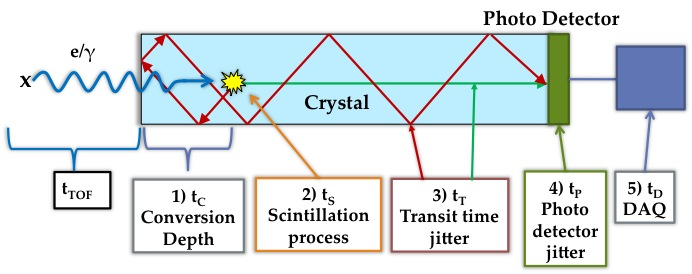
\includegraphics[width=0.85\textwidth]{figs/ScintillatorTiming} \caption{Factors
influencing the precision of the timing measurement with a monolithic, large
scintillating crystal. The incident particle impinges on the crystal face from
the left. Characteristic times of various factors are defined in the colored
boxes and in the text.}
\label{fig:ScintillatorTiming}
\end{figure}

The scintillation light produced needs to be detected. Typically this is done
with one or several photo detectors attached to the scintillator. The time $t_T$
it takes the scintillation photons to travel through the crystal may vary
substantially due to the isotropic angular distribution of the scintillation
light and the possible internal reflection of the light inside the crystal
before eventually reaching the photo detector. Finally, the photo detector and
its readout system have characteristic time constants $t_P$ and $t_D$ which will
affect the precision of the measurement as well.

In this study we focus on studying the effects of the shower development,
scintillation light emission and light propagation inside the crystal. Since the
photodetectors and readout system are shared with the experiment described
in~\cite{MCPFastCaloNIMA}, the chararacteristic times $t_P$ and $t_D$ are shared
between these two measurements. In our measurements in
Ref.~\cite{MCPFastCaloNIMA} we found the time-of-flight resolution between the
Photek 240 detectors to be $\sim 15$psec~\footnote{Here and in the following we
refer the standard deviation of the Gaussian fit as the ``resolution''}.
Assuming that the resolution of both Photek 240 is the same, one can derive the
time resolution of a Photek 240 to be $15/\sqrt{2}\approx$11 ps. The electronic
resolution of the DRS4 board was found to be $5-7$ psec. 

\begin{figure}[h] \centering
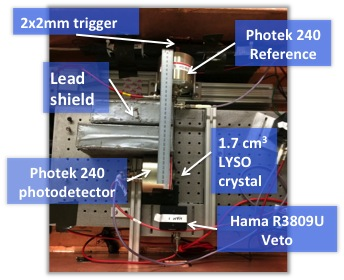
\includegraphics[width=0.5\textwidth]{figs/SetupLYSO} 
\caption{Experimental
setup for the test beam measurements. Inside a light tight box, shielded against
environmental noise, a LYSO crystal is mounted on one of the Photek 240
detectors. In all measurements the 2x2 mm$^2$ scintillator was used for
triggering. The reference Photek 240 is placed right after the trigger, and a
Hamamatsu R3809 MCP is placed behind the crystal as a Veto detector. Lead bricks
are placed upstream of the Photek 240 that reads out the crystal, to shield the detector from 
direct hits on MCP-PMT detector from beam particles.} 
\label{fig:SetupLYSO}
\end{figure}


In all results presented here which invoke the MCP based reference detector
measurement we did not unfold its contribution to the final result. In the
initial studies presented here we focus on measurements which allow to quantify
the contribution of the showering process in the crystals, the scintillation
light emission and the light propagation inside the crystal. These contributions
will dependent on the type of scintillator used, its size and its surface
properties. Future experiments will be carried out to study all these factors in
detail.

\section{Event Selection and Analysis}

\section{Time of Flight Resolution}

\section{Event Selection and Analysis}

\subsection{Sampling Calorimeter Setup}

\subsection{LYSO/W Shashlik Calorimeter Setup}

\section{Summary}

\end{document}  






























